\documentclass[11pt]{exam}
\usepackage[utf8]{inputenc}
\usepackage{hyperref}
\usepackage{graphicx}

\title{Reglas de Asociación en Weka}
\author{Laura Rodríguez Navas \\ rodrigueznavas@posgrado.uimp.es}
\date{\today}

\pagestyle{plain}

\begin{document}

\maketitle

En esta práctica se realiza un estudio acerca de los datos del hundimiento del Titanic a través de la herramienta \href{https://www.cs.waikato.ac.nz/ml/weka/}{Weka}. Los datos se encuentran en la dirección \url{http://www.hakank.org/weka/titanic.arff} y corresponden a las características de los 2201 pasajeros del Titanic. Estos datos son reales y se han obtenido de \textit{"Report on the Loss of the 'Titanic' (S.S.)" (1990), British Board of Trade Inquiry Report\_(reprint), Gloucester, UK: Allan Sutton Publishing}.

\vspace{3mm}

Para realizar esta práctica, se debe cargar el dataset Titanic que se ha descargado anteriormente y contestar a las siguientes preguntas:

\begin{questions}

% Pregunta 1
{\question Cuando ejecutamos el algoritmo Apriori de Weka, podemos utilizar diferentes umbrales de soporte. Dependiendo de qué umbrales de soporte pongamos, nos saldrán más o menos itemsets. Como resultado, Weka nos proporciona un conjunto de ítems L(1)... L(4) cuyos números van variando conforme cambiamos el umbral de soporte. 
	
Responde a las siguientes preguntas, utilizando capturas de pantalla y explicando los resultados de manera clara y concisa:}

\begin{parts}
\part ¿Qué representan cada uno de estos conjuntos de ítems? 

\renewcommand{\figurename}{Figura}

\begin{figure}[h]
	\centering
	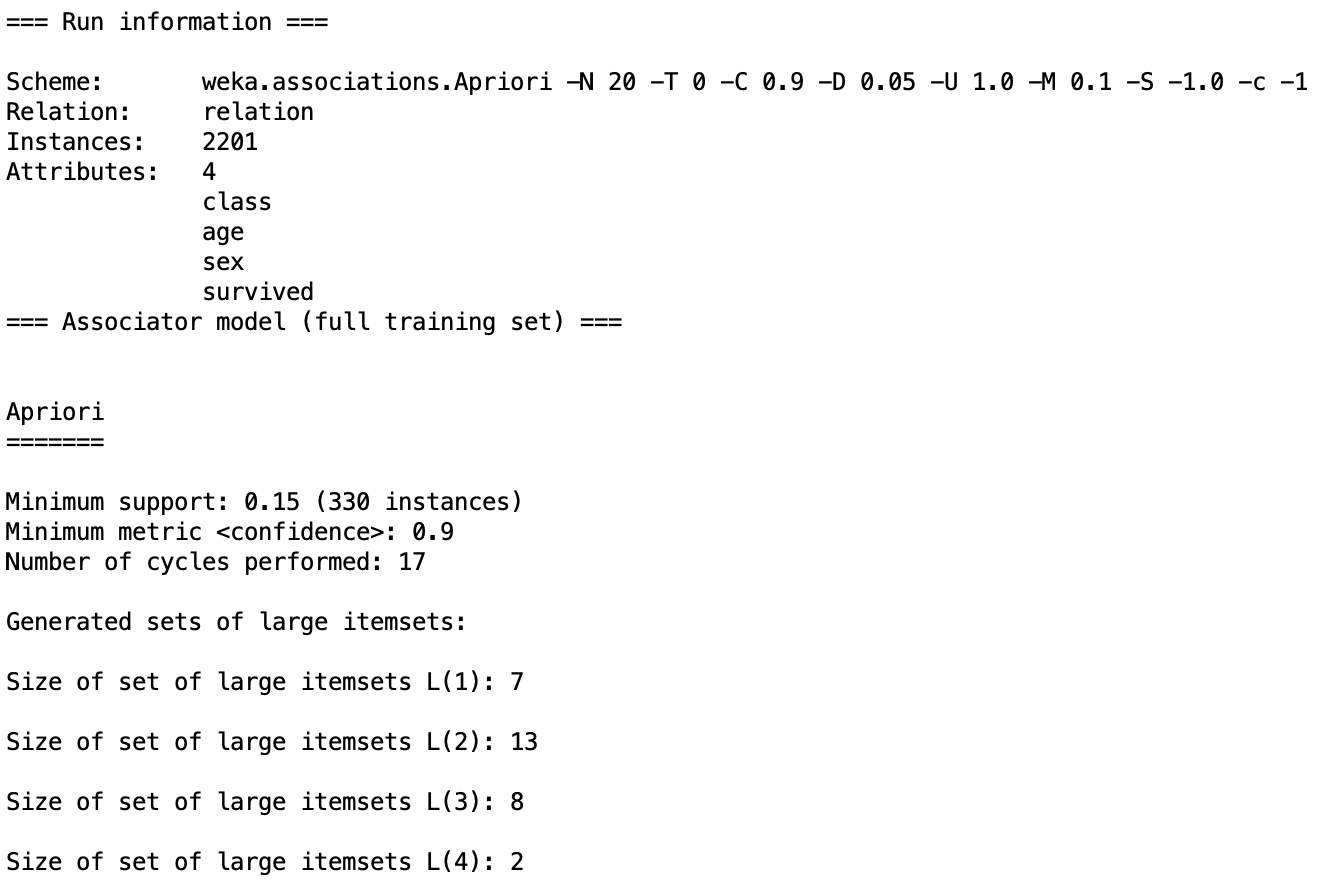
\includegraphics[scale=0.5]{Captura_1_1.png}
	\caption{soporte = 0.15 y confianza = 0.9.}
	\label{Captura_1_1}
\end{figure}

\begin{enumerate}
	\item El conjunto de ítems L(1) representa el número de conjuntos de ítems de tamaño 1. Que en este caso son 7.
	\item El conjunto de ítems L(2) representa el número de conjuntos de ítems de tamaño 2. Que en este caso son 13.
	\item El conjunto de ítems L(3) representa el número de conjuntos de ítems de tamaño 3. Que en este caso son 8.
	\item El conjunto de ítems L(4) representa el número de conjuntos de ítems de tamaño 4. Que en este caso son 2.
\end{enumerate}	

\part ¿Puede existir L(0)? Explica porqué.

No puede existir L(0). El conjunto de ítems L(0) representa el número de conjuntos de ítems de tamaño 0, es decir, el número de conjuntos de ítems vacíos, y el conjunto vacío ($\emptyset$) no es válido como conjunto de ítems.

\part ¿Puede existir L(5)? Explica porqué.

No puede existir L(5) porqué el dataset de Titanic solo contiene cuatro atributos diferentes. (ver Figura \ref{Captura_1_2}). 

\begin{figure}[h]
	\begin{center}
		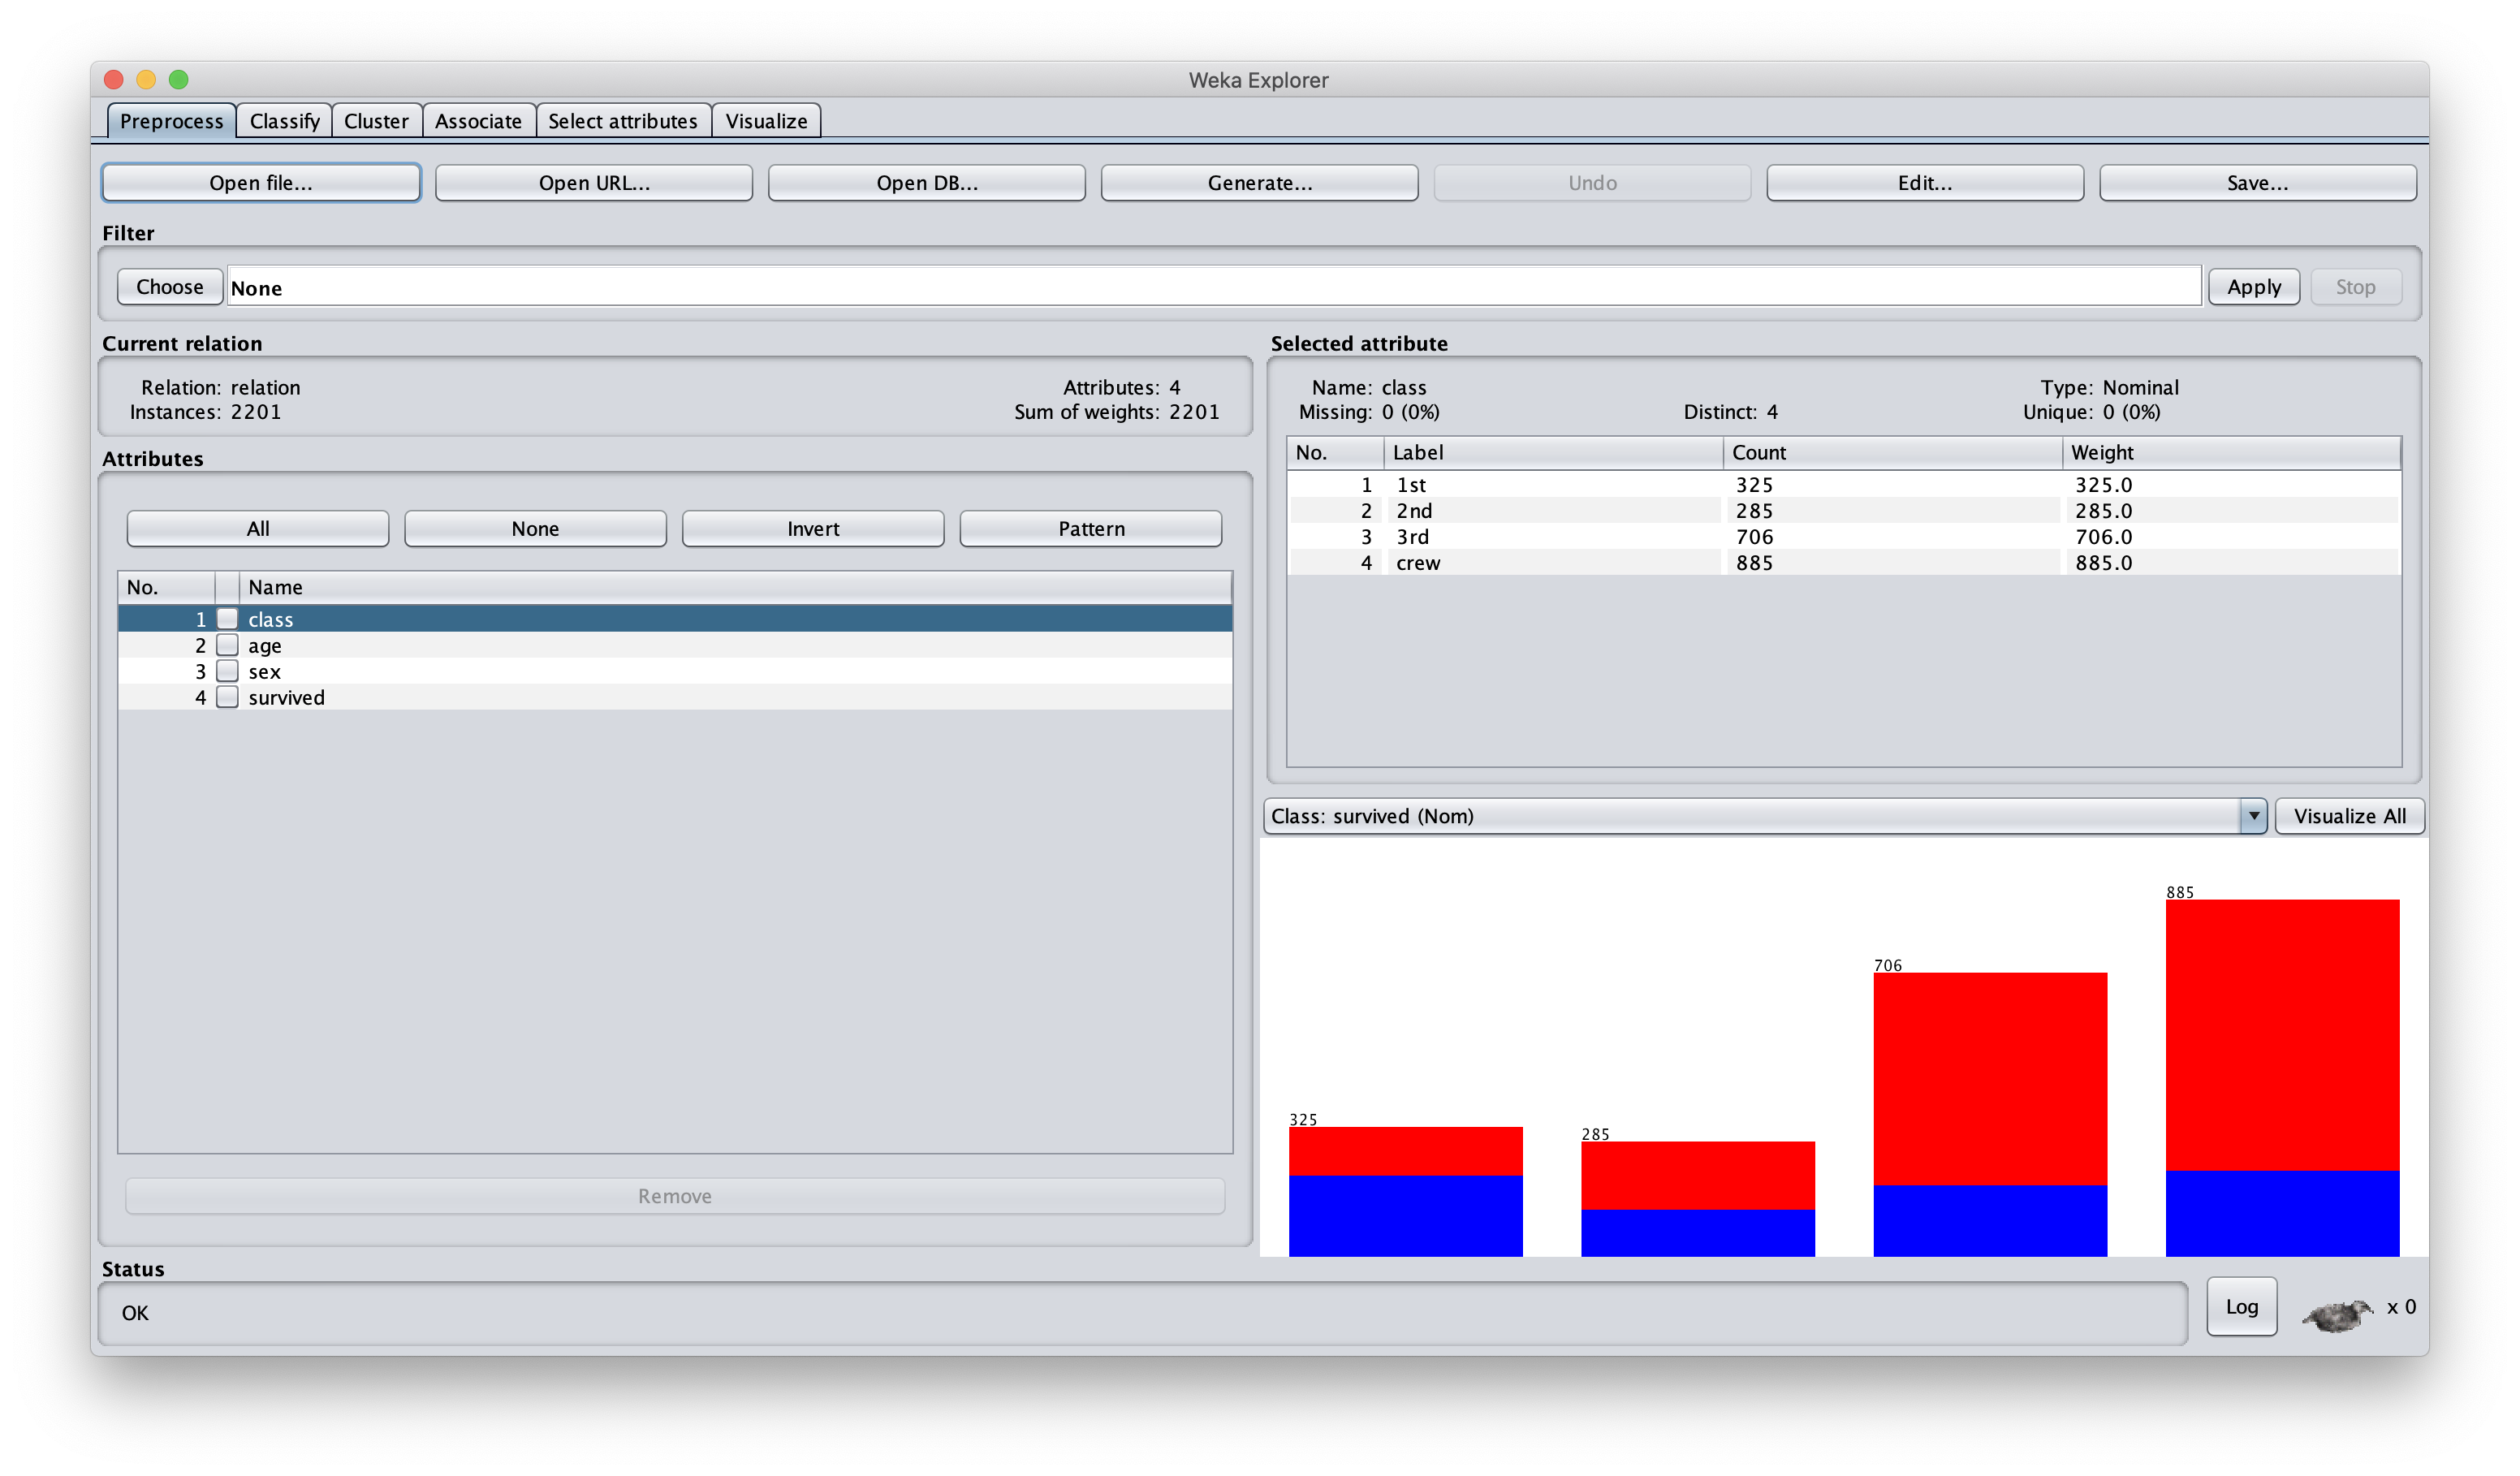
\includegraphics[scale=0.3]{Captura_1_2.png}
	\end{center}
\caption{características del dataset.}
\label{Captura_1_2}
\end{figure}

\part ¿Puede L(1) tomar un valor mayor que 10? Explica de manera teórica que eso no es posible y compruébalo experimentalmente.

L(1) no puede tomar un valor mayor que 10. El número de conjuntos de ítems de tamaño 1 será 9. Ya que, como máximo, el número de conjuntos de ítems de tamaño 1, cuenta con los diferentes valores de cada atributo del dataset. 

\newpage
En este caso, el dataset de Titanic, contiene 9 valores diferentes:

\begin{itemize}
	\item Class ("1st", "2nd", "3rd", "Crew")
	\item Age {"Adult", "Child"}
	\item Sex {"Male", "Female"}
	\item Survived {"Yes", "No"}
\end{itemize}

Para comprobarlo experimentalmente, el umbral de confianza debe ser igual a 1. (ver Figura \ref{Captura_1_3})

\begin{figure}[h]
	\centering
	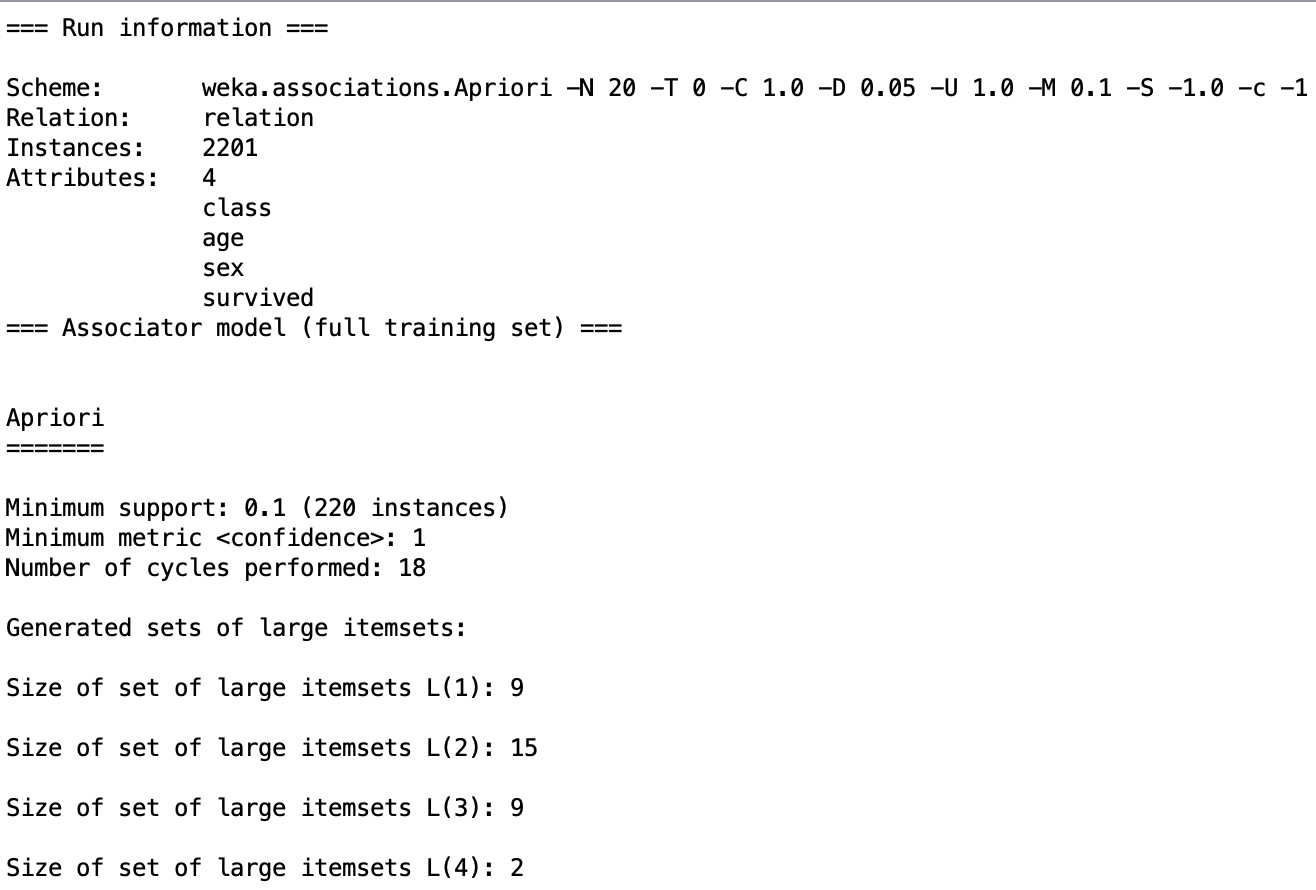
\includegraphics[scale=0.5]{Captura_1_3.png}
	\caption{soporte = 0.1 y confianza = 1.}
	\label{Captura_1_3}
\end{figure}

\end{parts}

% Pregunta 2
{\question Además de los valores de soporte, el algoritmo Apriori de Weka nos permite utilizar diferentes umbrales de soporte y confianza. Responde a las siguientes preguntas, utilizando capturas de pantalla y explicando los resultados de manera clara y concisa:}

\begin{parts}
\part ¿Es posible que una regla tenga un valor de soporte inferior a su confianza? Explica porqué y demuéstralo experimentalmente.

Sí. Lo podemos volver a ver en la Figura \ref{Captura_1_1}. Puede ser que la proporción de los conjuntos de ítems dentro del dataset sea alta y que la frecuencia co aparezca mucho en el dataset y la regla que contiene ese conjunto de datos tenga una frecuencia baja

\part ¿Es posible que una regla tenga un valor de confianza inferior a su suporte? Explica porqué y demuéstralo experimentalmente.

Sí, ver Figura \ref{Captura_1_4}.

\begin{figure}[h]
	\centering
	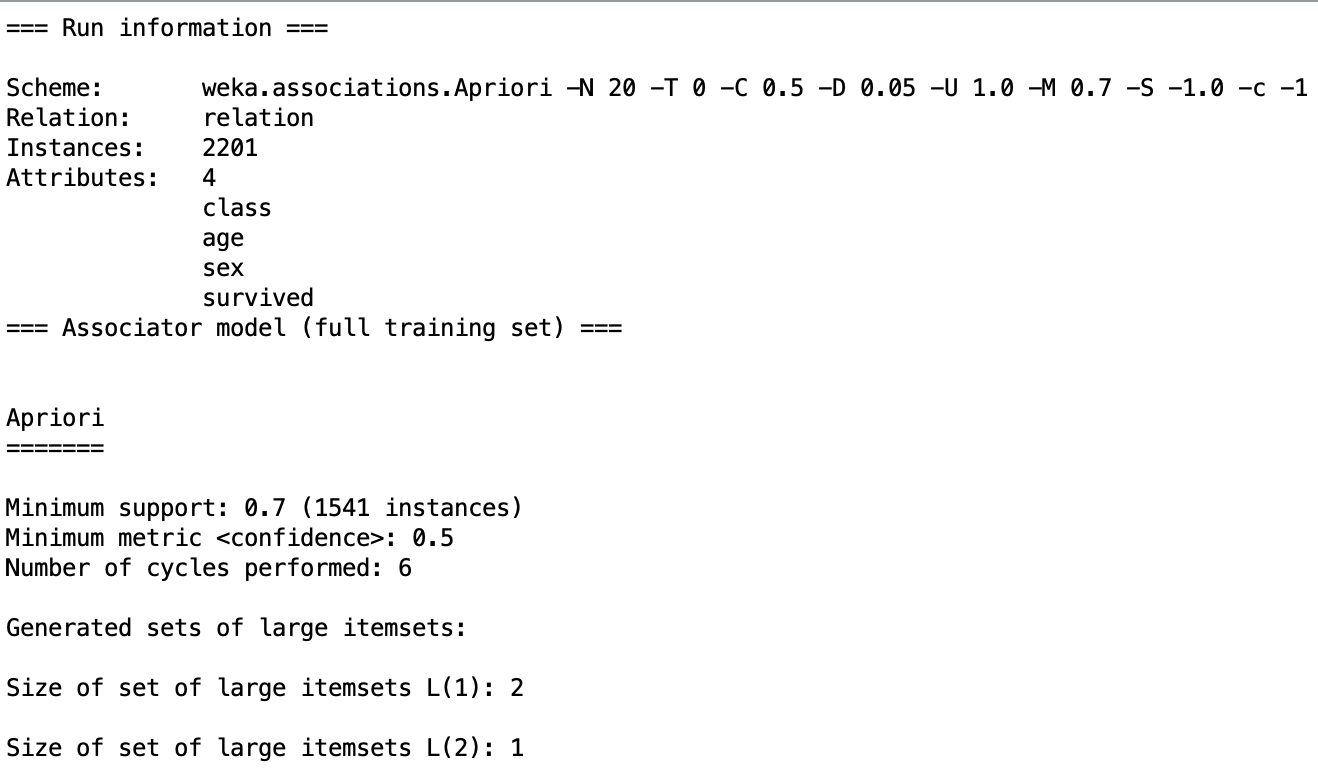
\includegraphics[scale=0.5]{Captura_1_4.png}
	\caption{Soporte = 0.7 y confianza = 0.5.}
	\label{Captura_1_4}
\end{figure}

\part La variación del umbral de confianza (dado un umbral fijo de soporte) no afecta a los conjuntos L(1)... L(4). ¿Por qué?
\end{parts}

Porqué la variación del umbral de confianza es una métrica enfocada para las reglas, y mide la frecuencia con que se pueden encontrar. En cambio, el umbral de soporte es una métrica enfocada para los conjuntos de ítems, que mide la proporción de estos dentro del dataset. Y como los  conjuntos L(1)... L(4) representan el número de apariciones de conjuntos de ítems según su tamaño dentro del dataset, el umbral les afectará.

% Pregunta 3
{\question Usaremos ahora, 0.75 como valor mínimo de soporte y de confianza 0.00. Comprobamos que obtenemos dos reglas de asociación, sin embargo, L(2) es 1. ¿Qué quiere decir esto? ¿A qué corresponde L(2)? ¿Qué itemset representa?}

Ver Figura \ref{Captura_1_5}.

\begin{figure}[h]
	\centering
	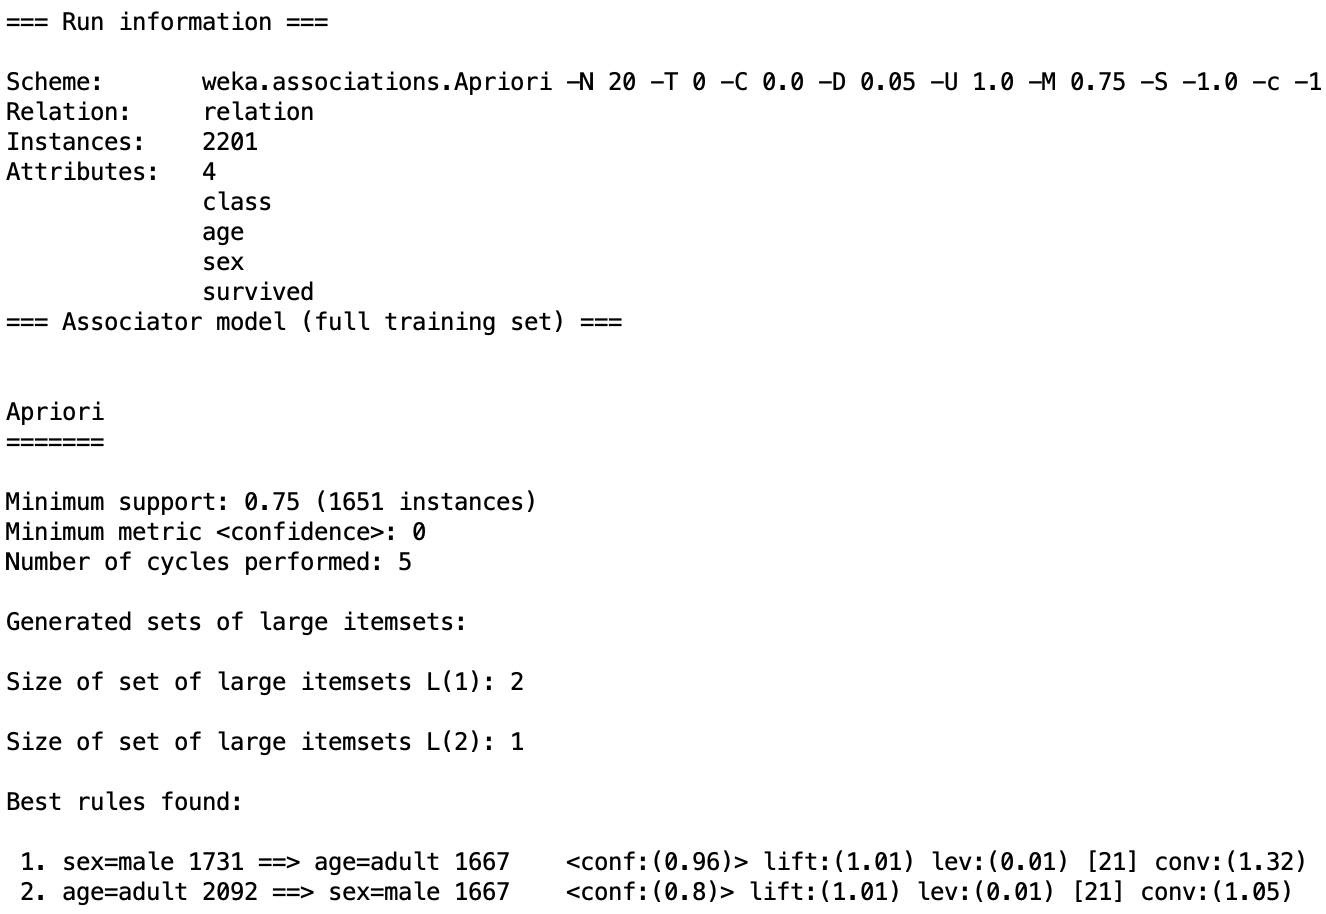
\includegraphics[scale=0.5]{Captura_1_5.png}
	\caption{Soporte = 0.75 y confianza = 0.}
	\label{Captura_1_5}
\end{figure}

% Pregunta 4
{\question Analiza el conjunto de reglas que salen al aplicar diferentes umbrales de soporte y confianza. Coge una regla, la que veas más interesante, y coméntala. Explica sus valores de métricas y qué representan, y el significado de la regla, es decir, el conocimiento que te aporta dicha regla.}

Después de aplicar diferentes umbrales de soporte y confianza la regla elegida es:
\end{questions}

\end{document}
